\section{Implementering}
\subsection{System Implementering}
Under implementeringen af nogle funktioner i samtlige moduler, er funktionerne efter følgende opstilling:\\

\methodDoc{Task\l T\g}{void}{async}{Foobar}{}

Funktionerne returnerer en Task af typen T og den kan gøres asynkron. Asynchrone metoder tillader programmet
at vente med at evaluere et functionskald indtil denne er helt færdig og dermed frigøre resourcer til andre
dele af programmet mens der vente på svar fra databasen.
Dette sker når en aynchron metode kaldes med ``await'' keywordet \\


\subsection{Frontend Implementering}
\label{Sec:FE-Implementering}
Til Frontend implementering er der brugt WPF med MVVM design patterns.
Til at skifte views uden at oprette et nyt vindue bruges et mediator design, hvor hver knap som skifter view giver en besked til mediatoren. Dette virker fordi alle views er oprettet som WPF user controls, og ikke views, hvilket tillader at et main view kan skifte mellem viewmodels, derved skifter alt indhold på vinduet, men uden at selve rammen skifter. Dette resulterer i et mere flydende User Interface for brugeren og derved en alt i alt bedre oplevelse. \cite{Mediator}\\
Et eksempel på hvordan mediatoren kaldes ved et tryk på en knap kan ses i følgende kode eksempel:

\begin{lstlisting}[language=c]
private DelegateCommand _loadGame;
    
public DelegateCommand LoadGame => _loadGame ?? (
	_loadGame = new DelegateCommand(
	ExecuteLoadCommand, CanExecuteLoadCommand));

async void ExecuteLoadCommand()
{
    await GameController.Instance.LoadGame(SelectedSave.ID);
    Mediator.Notify("GameStart", "");
}

bool CanExecuteLoadCommand()
{
    return SelectedSave != null;
}

void LoadCommand()
{
    LoadGame.RaiseCanExecuteChanged();
}
\end{lstlisting}

Visuelt er alle views implementeret tæt på det oprindelige design. Antallet og placering af knapper har ændret sig en smule, men den primære ide er uændret. Et eksempel på dette er room view.
For at se mere om hvordan andre views og menuer er implementeret se bilag \parencite[][Section 11.2]{TekniskBilag}

\subsubsection{Room View}

Visuelt er room view (\autoref{fig:Design-FE-impl-room}) ikke ændret betydeligt fra det oprindelige design. Der er ændret lidt på placering og antal af knapper så det passer til antallet af interaktioner tilgængelig til brugeren. Kortet er lavet så det opdateres når spilleren går ind i et nyt rum, ved at ændre på synligheden af elementerne i kortet. Det er yderligere sat op så det kan skaleres til de skærmopløsninger som understøttes.\\
Ved at trykke på interact knappen kan spilleren flytte et valgt 'item' fra listen nederst til venstre over i sit inventory (et seperat view), som kan tilgås ved at trykke på Inventory knappen.\\
Alt tekst er vist med data binding.

\begin{figure}[H]
\centering
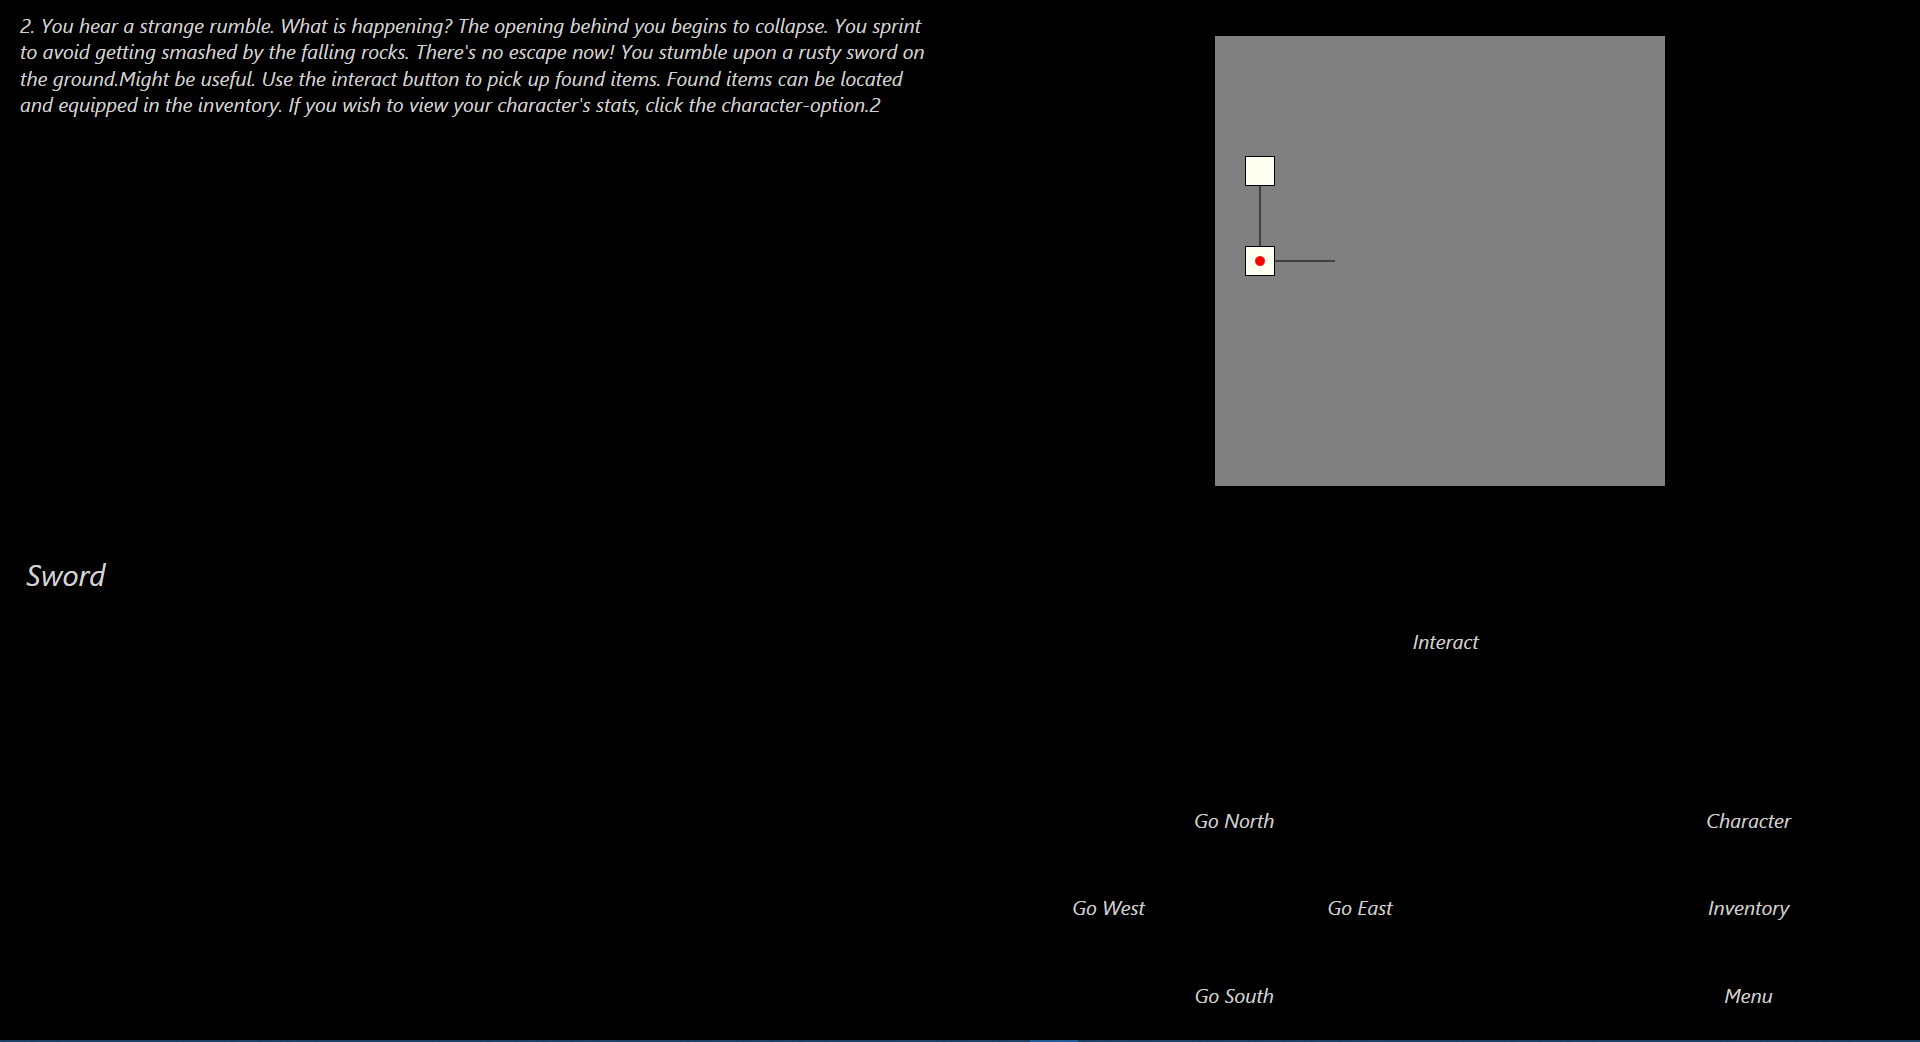
\includegraphics[width = \textwidth]{02-Body/Images/room_final.PNG}
\caption{Endeligt udseende af room view. Generelt er der ikke ændret meget i forhold til det oprindelige design. Kortet er lavet så det skalerer med skærmopløsningen.}
\label{fig:Design-FE-impl-room}
\end{figure}

\subsection{Game Engine}
Game Engine er implementeret i C\#, et objectorienteret programmeringsprog
med stærk library support, der tillader udvikling af applikationer. 
\autoref{fig:CoreDiagram} giver en klar indsigt i hvordan kernedelen af
game engine er designet til at virke. 

\subsubsection{Game Controller}
Game controlleren er det centrale komponent i game engine; ansvarlig for 
kommunikation med frontend modulet. Game controlleren har adgang til alle
aspekter af spillet, gennem sin association med Combat controlleren og 
backend controlleren.

\noindent Det er en nem løsning, og den fungerer godt givet det begrænsede scope som 
game enginen skal fungere under.
For en mere kompliceret applikation med forventninger om udvidelser er det
dog ikke en god implementering da game controlleren har for mange grunde
til at ændre sig. Den har altså et for bredt ansvarsområde og kan formentlig
splittes op i flere klasser.

\noindent Når game controlleren instantieres laves et map af Map og Map creator klassen
hvilket før til en længere process hvor map creator klassen laver nogle
layout filer som map klassen kan læse for at danne et map i spillet, som 
spilleren kan navigere \parencite[Section 11.3.2][]{TekniskBilag}.\\

\noindent Game controlleren er i stand til at save og load games gennem 
dens relation til backend controlleren, der kan lave fetch til spillets
database.

\noindent Selve Load process er kompliceret, da den involvere adskillige iterationer
igennem alle rooms, items og fjender i spillet for at bekræfte om disse er
blevet besøgt, indsamlet eller beseret tidligere \parencite[Section 11.3.1]
[Figure 55]{TekniskBilag}.
Save game er simplere, da game controlleren selv har adgang til alt infomation
som er nødvendigt for et komplet save game.

\subsubsection{Combat Controller}
Skulle spilleren befinde sig i combat, er det combat controlleren, der styre programmets
``flow of execution''. Først angriber spilleren; fjenden hvorefter fjenden angriber spilleren
hvis og kun hvis fjenden stadig er i live. Combat controlleren benytter en diceRoller til
at simulere terningekast, der benyttes til at bedømme om spilleren og fjenden rammer med
deres repektive angreb og efterfølgende; hvor meget deres angreb skader. Spilleren kan opsamle
og benytte våben til at forbedre deres terningekast \parencite[Section 10.3.2][]{TekniskBilag}. 

\subsubsection{Log}
Game Controlleren kommunikerer med front-end gennem en log. Loggen logger forskellige
events når game controlleren ændre game statet. Frontend kan derefter benytte loggen
til at læse og vise hvilket ændringer, der er foretaget og præsentere dem til spilleren
på en brugbar måde og brugervenlig måde.

\newpage

\subsection{Backend Implementering}

I det følgende afsnit gennemgåes implementerings detaljer omkring backendens controller klasser, samt BackEndController klassen på client siden. Alle controller klasserne er implementeret i C\#, da dette er sproget som anvendes i Asp.net Core. \\

\subsubsection{SaveController}
SaveController klassen inkluderer librariet Mircosoft.AspNetCore.MVC, dette gør det muligt, at anvende atributter til at definere hvilke Http metoder som funktionerne anvender eksempelvis HttpGet se \autoref{fig:Implementering-Backend-Code-GetSave}.

\begin{figure}[H]
\centering
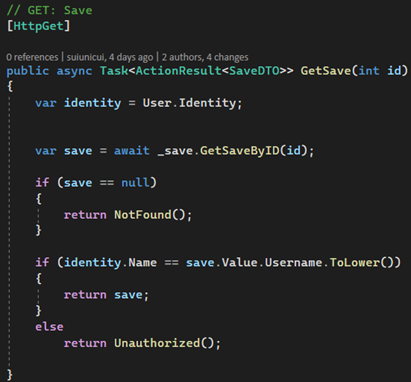
\includegraphics[width = 0.8\textwidth]{02-Body/Images/Backend_Code_GetSave.PNG}
\caption{Code snippet af HttpGet metode som modtager et id og retunere et SaveDTO object til clienten}
\label{fig:Implementering-Backend-Code-GetSave}
\end{figure}

Librariet gør det ligeledes muligt at retunere ActionResults, som kan indeholde objekter og en status kode eller blot en status kode, hvis noget går galt. Alle funktionerne er async og retunerer en Task, hvilket gør at der er tale om asynkrone funktioner, der først retunerer en værdi når dataen er klar. Dette gør også at clienten kan klare andre opgaver ind til dataen er klar.
SaveController inkluderer også Microsoft.AspNetCore.Authorization librariet, som bidrager med funktionalitet til kun at tilade kald, fra en korrekt bruger med Atributten [Authorize]. Da der kun findes en type af identiteter nemlig en helt normal bruger, som har adgang til alle endpoints, skal der findes en måde at sikre at brugeren kun kan tilgå sine egne data. Derfor gøres brug af User.Identity, kan ses på figur 10. Dette anvendes til at hente Claims User'eren tilhørende den nuværende action, hvilket så kan bruges til at tjekke om brugeren har lov til at hente det pågældende gemte spil.\\
    

\subsubsection{UserController}

UserController klassen minder meget om SaveController klassen, den gør ligeledes brug af Libraries Microsoft.AspNetCore.MVC og Microsoft.AspNetCore.Authorize. På \autoref{fig:Implementering-Backend-Code-Lgoin} ses Login funktionen.

\begin{figure}[H]
\centering
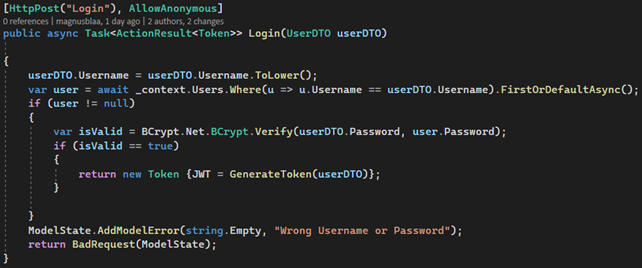
\includegraphics[width = \textwidth]{02-Body/Images/Backend_Code_Login.PNG}
\caption{Code snippet af HttpPost metode som modtager et UserDTO object og retunerer en JWT hvis brugeren findes og password’et er korrekt}
\label{fig:Implementering-Backend-Code-Lgoin}
\end{figure}

Her tilføjes endnu en attribut AllowAnonymous, da login skal være et anonymt kald, fordi brugeren endnu ikke er logget ind på clienten. Hvis brugeren findes og pasword'et er korrekt retuneres en ny JWT.\\

\subsubsection{BackEndController Client}
BackEndControlleren indeholde som det blev nævnt i backend Design afsnittet \autoref{ssec: Backend Design} et HttpClient objekt til at håndtere http request/response, og et Token objekt til at holde på den modtagne JWT.
Et klasse diagram over BackEndControlleren kan ses på \autoref{fig:Implementering-Backend-Klasse-BackEndController}\\

\begin{figure}[H]
\centering
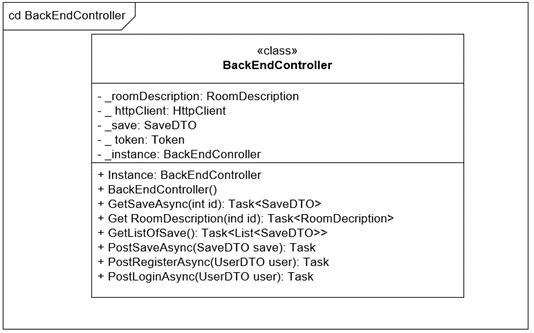
\includegraphics[width = \textwidth]{02-Body/Images/Backend_klasse_BackEndController.PNG}
\caption{klasse diagram af BackEndController}
\label{fig:Implementering-Backend-Klasse-BackEndController}
\end{figure}

For at sikre at der kun findes en JWT i programmet ad gangen, skal BackEndController klassen implementeres som en singleton, hvilket vil sige at der kun eksiterer en enkelt instance i hele programmet, som der er global adgang til. På den måde sikres det nemlig at BackEndController altid indeholder den korrekte JWT, uanset hvor henne i programmet der laves en request fra. Uden dette ville JWT nemlig kun være sat inde i det scope, hvor der blev logget ind eller en bruger blev registreret fra, altså der hvor den nuværende instance af BackendControlleren eksiterer. Funktionerne her er ligeledes asynkrone.\\


\subsubsection{Konlusion}

Funktionerne i backend controller klasserne samt funktionerne på clientens BackEndController er implementeret som asynkrone funktioner, der først retunerer en værdi når resourcen som efterspørges er klar. Client klassen er implementeret som en singleton for at holde styr på den aktuelle JWT.

\newpage

\subsection{Database Implementering}
\label{Section: DB-Implementering}
Til implementering og håndtering af databasen i .NET har gruppen valgt at benytte Entity framework core.
EF core gør det nemt at oprette og håndtere objekter C\# som skal gemmes eller hentes i databasen.\\
Til modellering af databasen benyttes det udarbejdede ER-diagram hvorpå keys og relations er bestemt.\\
Disse keys og relations opsættes i projektets backend ved hjælp af fluent api, hvori man nemt kan specificere keys, foreign keys, relations, hasData og meget mere.\\
Ved ændringer af databasens udseende og form kan EFcore migrations hjælpe med at oprette de korrekte queries således at databasen bliver ændret korrekt, samt at man ved forkerte ændringer hurtigt kan hoppe tilbage til en tidligere migration ved eventuelle fejl. I EF core benyttes Language Integrated Query (LINQ) til at skrive ensartede queries til databasen.\\

Der er i projektets backend oprettet klasser, models, tilsvarende ER diagrammernes entiteter. Udover det valgte atributter er der også oprettet navigationals i de nødvendige klasse så der kan laves relationer.
På \autoref{fig:DbKeys} herunder ses opsætningen af keys for de forskellige entiteter. Disse er opsat med fluent api efter ER diagrammerne på \autoref{fig:ER-Roomdescription} og \autoref{fig:ER-GameSave}.

\begin{figure}[H]
\centering
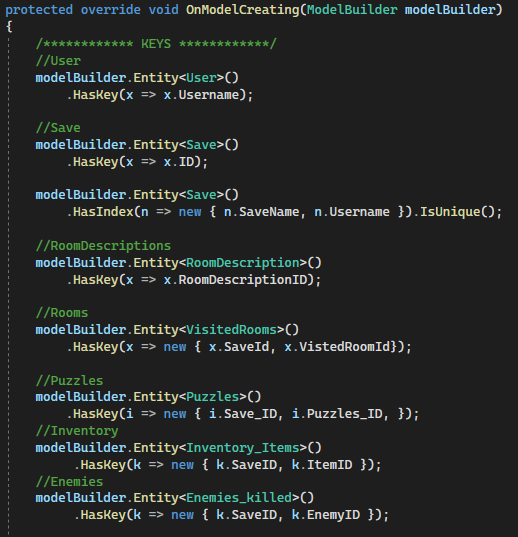
\includegraphics[width = 0.7\textwidth]{02-Body/Images/DAL-Database/DbKeys.PNG}
\caption{Opsætning af keys og unikke indexes for de forskellige entiteter i backends DbContext}
\label{fig:DbKeys}
\end{figure}

Udover de forskellige keys, skal der også opsættes relationer mellem de forskellige entiteter, som vist på ER-Diagrammerne \autoref{fig:ER-Roomdescription} og \autoref{fig:ER-GameSave}, samt referencer til foreign keys. 
Opsætningen kan ses på \autoref{fig:DbRelations} herunder: 

\begin{figure}[H]
\centering
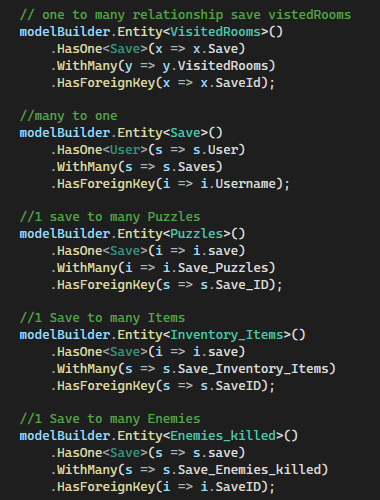
\includegraphics[width = 0.5\textwidth]{02-Body/Images/DAL-Database/DbRelations.PNG}
\caption{Opsætning af relations og foreign keys for de forskellige entiteter i backends DbContext}
\label{fig:DbRelations}
\end{figure}

Databasen er seedet ved hjælp af hasdata funktionen. Her oprettes en enkelt bruger, ”Gamer1”, med password ”123”, som hashes ind i databasen. "Gamer1" får derudover også 5 tilhørende "tomme" saves og til slut er der også indsat rumbeskrivelser for hver af de 20 rum. Dette ses på \autoref{fig:DbSeeding} herunder.

\begin{figure}[H]
\centering
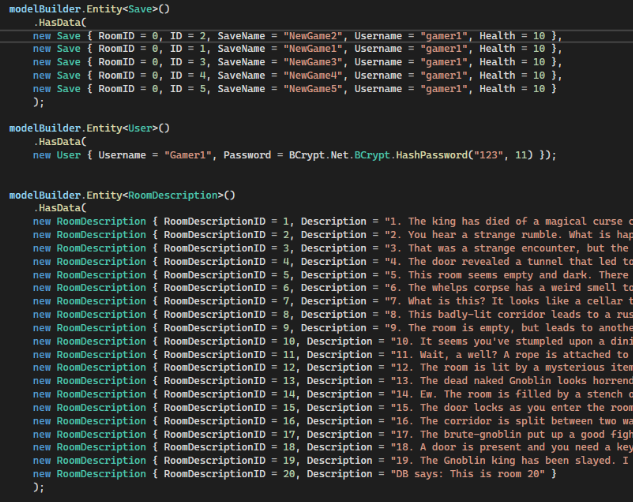
\includegraphics[width = 0.85\textwidth]{02-Body/Images/DAL-Database/DbSeeding.PNG}
\caption{Seeding af databasen med en enkel bruger, "Gamer1", 5 tilhørende "tomme" saves og beskrivelser af historien til de 20 forskellige rum}
\label{fig:DbSeeding}
\end{figure}
